\section{GUI Programming}

\subsection{Graphical User Interface (GUI)}
A GUI, pronounced as "gooey", stands for Graphical User Interface. The primary rationale behind GUIs is to enhance user experience by providing visual representations of program functions and data. GUIs enable users to interact with software applications through graphical elements like windows, buttons, menus, and icons, rather than relying solely on text-based commands.

GUI programming involves creating visually appealing interfaces for software applications using graphical elements like windows, buttons, and menus. Understanding basic GUI concepts and terminology is essential for developing user-friendly and intuitive applications.

\subsubsection{Visual Programming}
Visual programming involves creating applications using graphical elements rather than writing code manually. Examples of visual programming environments include Scratch, Blockly, and LabVIEW. These environments typically provide drag-and-drop interfaces for building applications, making it easier for users to create software without extensive programming knowledge.

\subsubsection{Widgets Toolkits}
Widget toolkits, also known as \textbf{GUI toolkits} or \textbf{frameworks}, provide libraries of reusable graphical components ("widgets") for building GUI applications. These toolkits offer APIs (Application Programming Interfaces) for creating and managing GUI elements, handling user interactions, and rendering graphical content. Examples of popular widget toolkits include Tkinter (for Python), Swing (for Java), WinForms (for .NET), and Qt (for C++ and Python).\\

\textbf{Widgets}, also known as controls, are graphical elements used in GUIs to interact with users or display information. Some basic terms associated with widgets include:

\begin{itemize}
    \item \textbf{Windows:} Rectangular areas on the screen that contain application content and controls.
    \item \textbf{Title and Title Bars:} The title of a window and the bar across the top of a window that contains the title and control buttons (minimize, maximize, close).
    \item \textbf{Buttons:} Controls that trigger actions when clicked, such as submitting a form or closing a window.
    \item \textbf{Icons:} Small graphical representations of files, folders, or applications.
    \item \textbf{Labels:} Text elements used to display static text or descriptions.
\end{itemize}

\subsubsection{Classical vs. Event-Driven Programming}
In classical programming, applications follow a sequential flow where each instruction is executed in order. In contrast, event-driven programming relies on events triggered by user actions or system events. Applications respond to these events by executing specific event-handling code. GUI programming is primarily event-driven, where user interactions such as clicking a button or typing in a text box trigger events that drive application behavior.\\

\textbf{Events} are actions or occurrences that happen during program execution, such as clicking a button, pressing a key, or moving the mouse. GUI applications respond to these events by executing event-handling code associated with each event type. Examples of events include mouse clicks, key presses, window resizing, and timer expiration.

\subsection{Tkinter}

\subsubsection{Simple Tkinter Application}
Tkinter is a Python library for creating GUI applications. It is the standard GUI toolkit for Python and is included with most Python installations, making it readily available for developers. Tkinter is based on the Tk GUI toolkit originally developed for the Tcl programming language.

\begin{codebox}
\begin{minted}{python}
import tkinter as tk

# Function to close the window
def close_window():
    root.destroy()

# Create the main Tkinter window
root = tk.Tk()
root.title("Simple Tkinter Application")

# Create a label widget
label = tk.Label(root, text="Hello, Tkinter!")
label.pack(pady=10)

# Create a button widget
close_button = tk.Button(root, text="Close", command=close_window)
close_button.pack()

# Start the Tkinter event loop
root.mainloop()
\end{minted}
\end{codebox}

\begin{figure}[h]
    \centering
    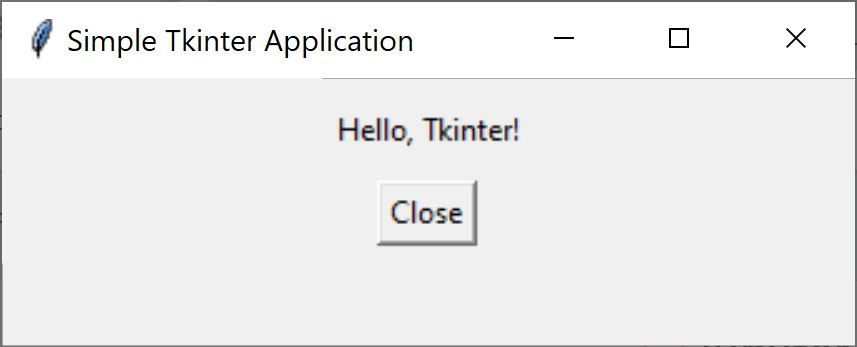
\includegraphics[width=0.6\textwidth]{images/tkinter1.JPG}
    \caption{Simple Tkinter Application}
    \label{fig:example}
\end{figure}

\subsubsection{The \texttt{mainloop()}}
In Tkinter, \texttt{mainloop()} is a method that runs an event loop, which listens for events such as user input (like mouse clicks and key presses) and system events. It's a fundamental part of any Tkinter application as it keeps the application running and responsive to user interactions.

\newpage
\subsubsection{Tkinter Widgets}

A widget is a graphical element or control used to display information or receive input in a GUI.

\begin{itemize}
    \item \textbf{Frame}: A container widget used to organize other widgets.
    
    \item \textbf{Label}: Displays text or images.
    
    \item \textbf{Button}: Generates an event when clicked.
    
    \item \textbf{Checkbutton}: Represents an on/off choice.
    
    \item \textbf{Radiobutton}: Allows the user to select one option from several.
    
    \item \textbf{Entry}: Accepts single-line text input from the user.
    
    \item \textbf{Combobox}: A combination of an Entry widget and a drop-down list.
    
    \item \textbf{Listbox}: Displays a list of items for selection.
    
    \item \textbf{Scrollbar}: Allows scrolling through content in widgets like Listbox or Canvas.
    
    \item \textbf{Sizegrip}: Provides a resize handle for resizable windows.
    
    \item \textbf{Text}: Multiline text editor.
    
    \item \textbf{Progressbar}: Displays the progress of a task.
    
    \item \textbf{Scale}: Represents a range of values as a slider.
    
    \item \textbf{Spinbox}: Input field with up/down buttons for numeric values.
    
    \item \textbf{Separator}: Horizontal or vertical line used to separate widgets.
    
    \item \textbf{Labelframe}: A frame with a title.
    
    \item \textbf{Panedwindow}: A container widget that holds panes (subwindows) split by a separator.
    
    \item \textbf{Notebook}: A tabbed notebook-like widget.
    
    \item \textbf{Canvas}: A drawing area for creating graphics and plots.
    
    \item \textbf{Treeview}: Displays hierarchical data in a tree-like structure.
\end{itemize}

\subsubsection{Widget Constructors}
A widget constructor is a method or function used to create an instance of a GUI component, typically known as a widget.

In frameworks like Tkinter (Python), JavaFX (Java), or PyQt (Python), GUI components like buttons, labels, text fields, etc., are created by calling specific constructor functions or methods provided by the framework. These constructor functions usually take parameters that define the initial properties or attributes of the widget, such as its size, position, text, color, etc. For example, in Tkinter, you might use the \texttt{Button} constructor to create a button widget.

\begin{codebox}
\begin{minted}{python}
import tkinter as tk

root = tk.Tk()

# Create a Button using the Button constructor
button = tk.Button(root, text="Click me", bg="red")

button.pack()

root.mainloop()
\end{minted}
\end{codebox}

\newpage
\subsubsection{Widget Properties and Methods}
Widget properties and methods provide essential functionalities for customizing and interacting with GUI elements in Tkinter.


\begin{itemize}
    \item \textbf{Common Properties}
    \begin{itemize}[label={--}]
        \item \texttt{text:} Sets or retrieves the text displayed by the widget.
        \item \texttt{bg:} Sets or retrieves the background color of the widget.
        \item \texttt{fg:} Sets or retrieves the foreground (text) color of the widget.
        \item \texttt{font:} Sets or retrieves the font used for the text in the widget.
        \item \texttt{width:} Sets or retrieves the width of the widget.
        \item \texttt{height:} Sets or retrieves the height of the widget.
        \item \texttt{state:} Sets or retrieves the state of the widget (normal, disabled, etc.).
        \item \texttt{variable:} Sets or retrieves the associated Tkinter variable.
    \end{itemize}

    \item \textbf{Common Methods}
    \begin{itemize}[label={--}]
        \item \texttt{config(**options):} Configures one or more widget options.
        \item \texttt{grid(**options):} Places the widget in the parent widget using a grid layout.
        \item \texttt{pack(**options):} Packs the widget into the parent widget.
        \item \texttt{place(**options):} Places the widget in the parent widget using absolute positioning.
        \item \texttt{focus():} Sets the keyboard focus to the widget.
        \item \texttt{bind(event, handler):} Binds an event to a handler function.
        \item \texttt{destroy():} Destroys the widget and removes it from the display.
    \end{itemize}
\end{itemize}


\newpage
\subsubsection{Positioning Widgets: \texttt{pack()} and \texttt{place()} and \texttt{grid()}}

In Tkinter, you can use various geometry managers to position widgets within a window. The most commonly used managers are \texttt{pack()}, \texttt{place()}, and \texttt{grid()}. If you want to position widgets within the interior of a window, you typically use the grid or place geometry managers.

\begin{itemize}
    \item \textbf{Pack Manager}
    \begin{itemize}
        \item Simple layout manager that arranges widgets in a block, either horizontally or vertically
        \item Widgets are packed into their parent container one after the other, vertically by default
        \item Options like side, fill, and expand control how widgets are packed and distributed within the available space
        \item Easy to use and suitable for most simple layouts
    \end{itemize}
    
    \item \textbf{Place Manager}
    \begin{itemize}
        \item Precise control over the position and size of widgets by specifying exact coordinates
        \item Positioning with absolute positioning rather than being packed in relation to each other
        \item More precise control but more complex to manage, especially with resizable windows
        \item Often used when you need pixel-perfect positioning or when arranging widgets relative to specific locations or other widgets
    \end{itemize}
    
        \item \textbf{Grid Manager}
    \begin{itemize}
           \item Divides the window into a grid of rows and columns.
    		   \item You can place widgets at specific row and column coordinates.
    		   \item Offers more control over widget positioning compared to the pack manager.
    \item Ideal for complex layouts.
    \end{itemize}
\end{itemize}

\subsubsection{Pack Manager Example}
This example demonstrates how to use the pack geometry manager in Tkinter to layout widgets within the application window. Widgets are packed against one side of the container, and in this example, we pack labels and buttons with padding between them.

\begin{codebox}
\begin{minted}{python}
import tkinter as tk

# Create the main application window
root = tk.Tk()
root.title("Pack Manager Example")

# Pack Manager Example
label1 = tk.Label(root, text="Label 1", bg="lightblue")
label1.pack(padx=10, pady=10)

button1 = tk.Button(root, text="Button 1", bg="lightcoral")
button1.pack(padx=10, pady=10)

# Start the Tkinter event loop
root.mainloop()
\end{minted}
\end{codebox}

\newpage
\subsubsection{Place Manager Example}
This example illustrates the usage of the place geometry manager, which allows precise positioning of widgets using absolute coordinates. Widgets are placed at specific \texttt{x} and \texttt{y} coordinates within the window. This manager provides fine-grained control over widget placement.

\begin{codebox}
\begin{minted}{python}
import tkinter as tk

# Create the main application window
root = tk.Tk()
root.title("Place Manager Example")

# Place Manager Example
label1 = tk.Label(root, text="Label 1", bg="lightblue")
label1.place(x=10, y=10)

button1 = tk.Button(root, text="Button 1", bg="lightcoral")
button1.place(x=10, y=40)

# Start the Tkinter event loop
root.mainloop()
\end{minted}
\end{codebox}

\subsubsection{Grid Manager Example}
This example demonstrates the grid geometry manager, which divides the window into a grid of rows and columns. Widgets are then placed at specific row and column coordinates within this grid. This manager provides more control over widget positioning compared to \texttt{pack()}.

\begin{codebox}
\begin{minted}{python}
import tkinter as tk

# Create the main application window
root = tk.Tk()
root.title("Grid Manager Example")

# Create widgets and place them using the grid manager
label1 = tk.Label(root, text="Label 1", bg="lightblue")
label1.grid(row=0, column=0, padx=10, pady=10)

label2 = tk.Label(root, text="Label 2", bg="lightgreen")
label2.grid(row=1, column=0, padx=10, pady=10)

button1 = tk.Button(root, text="Button 1", bg="lightcoral")
button1.grid(row=0, column=1, padx=10, pady=10)

button2 = tk.Button(root, text="Button 2", bg="lightyellow")
button2.grid(row=1, column=1, padx=10, pady=10)

# Start the Tkinter event loop
root.mainloop()
\end{minted}
\end{codebox}

\newpage
\subsubsection{Screen Coordinates}
Screen coordinates refer to the position of elements relative to the display screen. They are typically expressed as a pair of integers representing the horizontal (x) and vertical (y) distances from a reference point, often the top-left corner of the screen.
\begin{codebox}
\begin{minted}{python}
import tkinter as tk

root = tk.Tk()

# Get the screen width and height
screen_width = root.winfo_screenwidth()
screen_height = root.winfo_screenheight()

print("Screen width:", screen_width)
print("Screen height:", screen_height)

root.mainloop()
\end{minted}
\end{codebox}
\subsubsection{Positioning and Sizing Windows}
Positioning and sizing windows in GUIs involves specifying their location and dimensions on the screen. This is typically achieved using screen coordinates for positioning and width and height values for sizing. To center a Tkinter window on the screen, you can calculate the coordinates for the top-left corner of the window based on the screen dimensions and the size of your window.
\begin{codebox}
\begin{minted}{python}
import tkinter as tk

def center_window(window, width, height):
    screen_width = window.winfo_screenwidth()
    screen_height = window.winfo_screenheight()
    
    x = (screen_width - width) // 2
    y = (screen_height - height) // 2
    
    window.geometry(f"{width}x{height}+{x}+{y}")

root = tk.Tk()

# Set the width and height of the window
window_width = 400
window_height = 300

# Center the window on the screen
center_window(root, window_width, window_height)

root.mainloop()
\end{minted}
\end{codebox}

Positioning elements using screen width involves calculating coordinates relative to the screen's width rather than fixed pixel values. By utilizing screen width-based positioning, developers can create responsive and adaptable layouts that adjust dynamically based on the screen's dimensions.

\newpage


\newpage
\subsubsection{Event Controllers}
Event controllers, also known as \textbf{event handlers} or \textbf{event listeners}, are components of software systems responsible for managing and responding to various user actions or system events. In GUIs, event controllers play a crucial role in capturing user interactions with the interface elements and triggering actions or responses.

\begin{itemize}
    \item \textbf{Callback functions}
    \begin{itemize}
        \item Callbacks are passed as an argument to another function or method. The purpose of a callback function is to be executed at a later time, often in response to a specific event or condition.
        \item In GUIs callback functions are commonly used to handle events triggered by user interactions with GUI elements such as buttons, menus, or input fields. These functions are passed as arguments to event-binding methods like \texttt{command} for buttons or \texttt{bind} for other widgets.
        \item When the associated event occurs (e.g., a button click), the callback function is invoked or called and executes the specified code or behavior.
    \end{itemize}
    
    \item \textbf{Closing a window with \texttt{destroy()}}
    \begin{itemize}
        \item The \texttt{destroy()} method is used to destroy or close a window or widget. When called on a Tkinter widget, such as a window (\texttt{Tk}) or a frame (\texttt{Frame}), it removes the widget and all its child widgets from the screen and releases associated system resources.
        \item Typically, \texttt{destroy()} is used in response to a specific condition or event, such as when the user closes a window or when a certain action is completed.
        \item When a window is destroyed, the main event loop (\texttt{mainloop()}) exits, and the program terminates.
    \end{itemize}
    
\end{itemize}

\begin{codebox}
\begin{minted}{python}
import tkinter as tk

# Event controller for click button
def click_button():
    print("Button clicked!")  # Callback function for click button

# Event controller for destroy button
def close_window():
    root.destroy()  # Callback function for destroy button

root = tk.Tk()

# Create a button to trigger the close_window callback
click_button = tk.Button(root, text="Click Button", command=click_button)
click_button.pack(padx=20, pady=20)

# Create a button to trigger the close_window callback
destroy_button = tk.Button(root, text="Destroy Button", command=close_window)
destroy_button.pack(padx=20, pady=20)

root.mainloop()
\end{minted}
\end{codebox}

\newpage
\subsubsection{Binding Events with \texttt{bind()}}
The \texttt{bind()} method is used to associate an event with a function. This method allows you to specify what should happen when a particular event occurs on a widget, such as a mouse click, a key press, or a mouse movement.

Mouse button events are represented by strings in a specific format.

\begin{itemize}
    \item \texttt{<Button-1>} represents the left mouse button being clicked.
    \item \texttt{<Button-2>} represents the middle mouse button (if present) being clicked.
    \item \texttt{<Button-3>} represents the right mouse button being clicked.
\end{itemize}

\begin{codebox}
\begin{minted}{python}
import tkinter as tk

def on_button_click(event):
    print("Button Clicked")

def on_button_release(event):
    print("Button Released")

def on_mouse_enter(event):
    print("Mouse Entered")

def on_mouse_leave(event):
    print("Mouse Left")

root = tk.Tk()
root.title("Identifying and Deriving Events")

# Create a button widget
button = tk.Button(root, text="Click Me")
button.pack(pady=20)

# Bind functions to identify button events
button.bind("<Button-1>", on_button_click)
button.bind("<ButtonRelease-1>", on_button_release)

# Bind functions to identify mouse events
button.bind("<Enter>", on_mouse_enter)
button.bind("<Leave>", on_mouse_leave)

root.mainloop()
\end{minted}
\end{codebox}

\newpage
\subsubsection{Dialogs}
Dialog boxes are GUI components used to interact with the user and request information or confirmation within an application. They typically appear as pop-up windows and can serve various purposes such as displaying messages, prompting for input, or confirming actions. In Tkinter, different types of dialog boxes can be created using built-in functions from the \texttt{tkinter.messagebox} module.\\

\begin{itemize}
    \item \textbf{Message Box} \\
    Displays a message and an OK button.
    \vspace{0.2cm}
    \begin{codebox}
    \begin{minted}{python}
import tkinter.messagebox as mb
mb.showinfo("Title", "Message")
    \end{minted}
    \end{codebox}
    \vspace{0.3cm}
    
    \item \textbf{Warning Box} \\
    Displays a warning message and an OK button.
    \vspace{0.2cm}
    \begin{codebox}
    \begin{minted}{python}
import tkinter.messagebox as mb
mb.showwarning("Title", "Warning Message")
    \end{minted}
    \end{codebox}
    \vspace{0.3cm}
    
    \item \textbf{Error Box} \\
    Displays an error message and an OK button.
    \vspace{0.2cm}
    \begin{codebox}
    \begin{minted}{python}
import tkinter.messagebox as mb
mb.showerror("Title", "Error Message")
    \end{minted}
    \end{codebox}
    \vspace{0.3cm}
    
    \item \textbf{Question Box} \\
    Displays a question and provides options for the user to respond with "Yes", "No", "Cancel", or other custom buttons.
    \vspace{0.2cm}
    \begin{codebox}
    \begin{minted}{python}
import tkinter.messagebox as mb
response = mb.askquestion("Title", "Question")
    \end{minted}
    \end{codebox}
    \vspace{0.3cm}
    
    \item \textbf{OK/Cancel Box} \\
    Asks the user to confirm or cancel an action.
    \vspace{0.2cm}
    \begin{codebox}
    \begin{minted}{python}
import tkinter.messagebox as mb
response = mb.askokcancel("Title", "Question")
    \end{minted}
    \end{codebox}
    \vspace{0.3cm}
    
    \item \textbf{Yes/No Box} \\
    Asks the user to respond with "Yes" or "No".
    \vspace{0.2cm}
    \begin{codebox}
    \begin{minted}{python}
import tkinter.messagebox as mb
response = mb.askyesno("Title", "Question")
    \end{minted}
    \end{codebox}
    \vspace{0.3cm}
    
    \item \textbf{Retry/Cancel Box} \\
    Asks the user to retry or cancel an operation.
    \vspace{0.2cm}
    \begin{codebox}
    \begin{minted}{python}
import tkinter.messagebox as mb
response = mb.askretrycancel("Title", "Question")
    \end{minted}
    \end{codebox}
    \vspace{0.3cm}
\end{itemize}

\newpage

\subsubsection{Validity of User Input}
Validating user input and handling errors are essential aspects of creating robust and user-friendly applications. 
\begin{codebox}
\begin{minted}{python}
import tkinter as tk
from tkinter import messagebox

def validate_number():
    try:
        value = float(entry.get())
        if value < 0 or value > 100:
            raise ValueError("Value must be between 0 and 100")
        messagebox.showinfo("Success", "Input is valid")
        entry.delete(0, tk.END)  # Clear input if valid
    except ValueError as e:
        messagebox.showerror("Error", str(e))
        entry.delete(0, tk.END)

root = tk.Tk()
root.title("Input Validation Example")

label = tk.Label(root, text="Enter a number between 0 and 100:")
label.pack(pady=10)

entry = tk.Entry(root)
entry.pack(pady=5)

validate_button = tk.Button(root, text="Validate", command=validate_number)
validate_button.pack(pady=5)

root.mainloop()
\end{minted}
\end{codebox}

\newpage
\subsubsection{Canvas}
A canvas is a widget that provides a drawing surface for creating graphics, diagrams, and other visual elements. It allows you to draw lines, shapes, text, images, and more using various methods and options.

\begin{codebox}
\begin{minted}{python}
import tkinter as tk

def draw_rectangle():
	# Draw a blue rectangle
    canvas.create_rectangle(50, 50, 150, 150, fill="blue")  

root = tk.Tk()
root.title("Canvas Example")

# Create a canvas widget
canvas = tk.Canvas(root, width=200, height=200, bg="white")
canvas.pack()

# Draw a rectangle on the canvas when a button is clicked
draw_button = tk.Button(root, text="Draw Rectangle", command=draw_rectangle)
draw_button.pack(pady=10)

root.mainloop()
\end{minted}
\end{codebox}

The canvas widget in Tkinter provides several methods for drawing and manipulating graphics on the canvas. Here are some commonly used canvas methods:

\begin{itemize}
    \item \texttt{create\_line(x1, y1, x2, y2, ...)}:
    Draws a straight line segment between the points \texttt{(x1, y1)} and \texttt{(x2, y2)}, and so on.
    
    \item \texttt{create\_rectangle(x1, y1, x2, y2, ...)}:
    Draws a rectangle with the top-left corner at \texttt{(x1, y1)} and the bottom-right corner at \texttt{(x2, y2)}.
    
    \item \texttt{create\_oval(x1, y1, x2, y2, ...)}:
    Draws an oval or circle inscribed within the rectangle defined by the top-left corner at \texttt{(x1, y1)} and the bottom-right corner at \texttt{(x2, y2)}.
    
    \item \texttt{create\_polygon(x1, y1, x2, y2, ..., options)}:
    Draws a polygon with vertices specified by alternating $x$ and $y$ coordinates.
    
    \item \texttt{create\_text(x, y, ...)}:
    Draws text at the specified coordinates \texttt{(x, y)}.
    
    \item \texttt{create\_image(x, y, ...)}:
    Displays an image at the specified coordinates \texttt{(x, y)}.
    
    \item \texttt{move(item, dx, dy)}:
    Moves the specified item (e.g., line, shape, text) by the specified delta values \texttt{(dx, dy)}.
    
    \item \texttt{delete(item)}:
    Deletes the specified item from the canvas.
    
    \item \texttt{itemconfig(item, ...)}:
    Modifies the configuration options of the specified item.
    
    \item \texttt{bind(sequence, callback)}:
    Binds an event (e.g., mouse click, key press) to a callback function for the canvas.
\end{itemize}

\newpage
\subsubsection{Coloring Widgets}

Coloring widgets in Tkinter enables customization of various elements such as labels, buttons, frames, etc., to align with the desired design of a graphical user interface (GUI). Both the background color (bg) and the foreground color (fg) of widgets can be specified.

\begin{codebox}
\begin{minted}{python}
import tkinter as tk

root = tk.Tk()
root.title("Color Example")
root.geometry("250x100")

# Set background color for the entire window
root.configure(bg="lightcoral")

# Label with default colors
label_default = tk.Label(root, text="Label", bg="darkblue", fg="green")
label_default.pack(padx=10, pady=10)

# Label with hexadecimal color
label_hex = tk.Label(root, text="Hex Label", bg="#00008B", fg="#90EE90")
label_hex.pack(padx=10, pady=10)

root.mainloop()
\end{minted}
\end{codebox}

\begin{itemize}
    \item \textbf{Default Color Names}
    \begin{itemize}
        \item Tkinter provides a set of predefined color names, allowing you to easily select colors without specifying specific color codes.
        \item For example, "red", "blue", "lightblue", etc., are recognized color names in Tkinter.
        \item These names correspond to common colors and simplify the process.
    \end{itemize}

    \item \textbf{Hexadecimal Color Codes}
    \begin{itemize}
        \item Hexadecimal color codes represent colors using a combination of six hexadecimal digits.
        \item Each pair of digits corresponds to the intensity of the red, green, and blue components.
        \item For example, \#FF0000 represents pure red, \#00FF00 represents pure green, and \#0000FF represents pure blue.
        \item Hexadecimal color codes provide a wide range of color options.
    \end{itemize}

    \item \textbf{RGB Values}
    \begin{itemize}
        \item RGB (Red, Green, Blue) values specify colors based on the intensity of red, green, and blue light components.
        \item Each component's intensity is represented by a value between 0 and 255.
        \item For example, (255, 0, 0) represents pure red, (0, 255, 0) represents pure green, and (0, 0, 255) represents pure blue.
        \item Tkinter does \textbf{NOT} directly support specifying colors using RGB values. RGB values must be converted to hexadecimal format for use in Tkinter.

    \end{itemize}
\end{itemize}

\subsubsection{Variables}
In Tkinter, variables are often used to link GUI elements (like widgets) with application data. The common variable types used are \texttt{StringVar}, \texttt{IntVar}, \texttt{DoubleVar}, and \texttt{BooleanVar}, each corresponding to a specific data type.\\

\textbf{Observable variables}, also known as observable objects or observable properties, are data structures that notify their observers when their internal state changes. These variables represent the state of GUI elements (such as widgets or components), and they allow other parts of the application to react to changes in this state.\\

In scenarios where you need to decouple components of an application observable variables can be useful. For example, in a GUI application, observable variables can represent the state of various GUI elements (like checkboxes, text fields, etc.), and different parts of the application can react to changes in these elements without directly coupling to each other.

\begin{codebox}
\begin{minted}{python}
from tkinter import Tk, Button, StringVar
 
root = Tk()
root.geometry('200x200')
 
str_var = StringVar()
str_var.set("Hello, Tkinter!")
 
def update_text():
    str_var.set("Button clicked!")

button = Button(root, textvariable=str_var, command=update_text)
button.pack()
 
root.mainloop()
\end{minted}
\end{codebox}

In Tkinter, \texttt{textvariable} is a configuration option available for specific widgets, including \texttt{Button}, \texttt{Label}, \texttt{Entry}, \texttt{Checkbutton}, and \texttt{Radiobutton}. It enables you to connect a Tkinter variable (such as \texttt{StringVar}, \texttt{IntVar}, etc.) with the widget's content. Consequently, when the linked variable's value changes, the widget's content automatically updates accordingly, and vice versa.\\


The text on the button changes to "Button clicked!". Using the \texttt{textvariable} option in Tkinter allows you to dynamically update the text of a widget by associating it with a tkinter variable such as \texttt{StringVar()}. This can be particularly useful when you want to update the text displayed on a button dynamically. 

\newpage
\begin{codebox}
\begin{minted}{python}
import tkinter as tk

class ObservableVariable:
    def __init__(self):
        self._value = ""
        self._observers = []

    def get(self):
        return self._value

    def set(self, value):
        self._value = value
        self.notify_observers()

    def add_observer(self, observer):
        self._observers.append(observer)

    def remove_observer(self, observer):
        self._observers.remove(observer)

    def notify_observers(self):
        for observer in self._observers:
            observer(self._value)

root = tk.Tk()
root.title("Observable Function in Tkinter")

observable_var = ObservableVariable()

# Function to be called whenever the input changes
def input_changed(new_value):
    print("Input changed:", new_value)

# Entry widget
entry = tk.Entry(root)
entry.pack(pady=10, padx=10)

# Bind the input_changed function to the observable variable
observable_var.add_observer(input_changed)

# Function to update the observable variable when the entry content changes
def update_variable(*args):
    new_value = entry.get()
    observable_var.set(new_value)

# Bind the update_variable function
entry.bind("<KeyRelease>", update_variable)

root.mainloop()
\end{minted}
\end{codebox}

\newpage

\subsubsection{Radiobuttons}
Radio buttons are a type of GUI element that allows users to select one option from a set of mutually exclusive options. They are typically used in forms, settings, and preference panels where users need to make a single selection from a list of choices.

\begin{codebox}
\begin{minted}{python}
import tkinter as tk

root = tk.Tk()
root.title("Radio Button Example")
root.geometry("300x150")
root.config(pady=10)

def on_change():
    selected = selected_option.get()
    label.config(text="Selected: " + selected)

# Variable to hold the selected radio button
default_selected = "None"
selected_option = tk.StringVar(value=default_selected)

# Create radio buttons in a loop
options=["Option 1","Option 2", "Option 3"]
for o in options:
    rb = tk.Radiobutton(root, 
                        text=o, 
                        value=o, 
                        variable=selected_option,
                        command=on_change)
    rb.pack(anchor=tk.W)

label = tk.Label(text="Selected: " + default_selected)
label.pack(pady=10)

root.mainloop()
\end{minted}
\end{codebox}

In the context of the radio buttons, \texttt{rb.pack(anchor=tk.W)} means that each radio button will be anchored to the west (left) side of its allocated space. This parameter is optional.

\begin{itemize}
    \item \textbf{\texttt{text}:}
    The \texttt{text} parameter in a \texttt{Radiobutton} widget specifies the label text that will be displayed alongside the radio button. Each radio button typically represents an option, and \texttt{text} is what labels that option.
    
    \item \textbf{\texttt{value}:}
    In a \texttt{Radiobutton} widget, the \texttt{value} parameter sets the value associated with that particular radio button. When a user selects a radio button, the corresponding value is assigned to the variable associated with the group of radio buttons.
    
    \item \textbf{\texttt{variable}:}
    The \texttt{variable} parameter in a \texttt{Radiobutton} widget associates a \texttt{StringVar}, \texttt{IntVar}, or \texttt{BooleanVar} variable with a group of radio buttons. This association ensures that only one radio button in the group can be selected at a time. When a radio button is selected, its value is stored in the associated variable.
    
    \item \textbf{\texttt{command}:}
    The \texttt{command} parameter in a \texttt{Radiobutton} widget specifies a function that will be called when the radio button is selected. This function typically performs some action in response to the selection of the radio button.
\end{itemize}

\subsubsection{Checkboxes}
Checkboxes are GUI elements used to allow users to make multiple selections from a set of options. They are used when users need to make one or more selections from a list of options. They are commonly used in forms, preference panels, settings, and other interfaces where users need to indicate their choices among multiple options.

\begin{codebox}
\begin{minted}{python}
import tkinter as tk

def show_checkbox_state():
    if check_var.get() == 1:
        status_label.config(text="Checkbox is checked")
    else:
        status_label.config(text="Checkbox is unchecked")

root = tk.Tk()
root.title("Checkbox Example")
root.geometry("300x150")

# Variable to hold the state of the checkbox
check_var = tk.IntVar()

# Create a checkbox
checkbox = tk.Checkbutton(root, 
                          text="Check me", 
                          variable=check_var, 
                          command=show_checkbox_state)
checkbox.pack(pady=30)

# Label to display the status of the checkbox
status_label = tk.Label(root, text="")
status_label.pack()

root.mainloop()
\end{minted}
\end{codebox}

\begin{figure}[h]
    \centering
    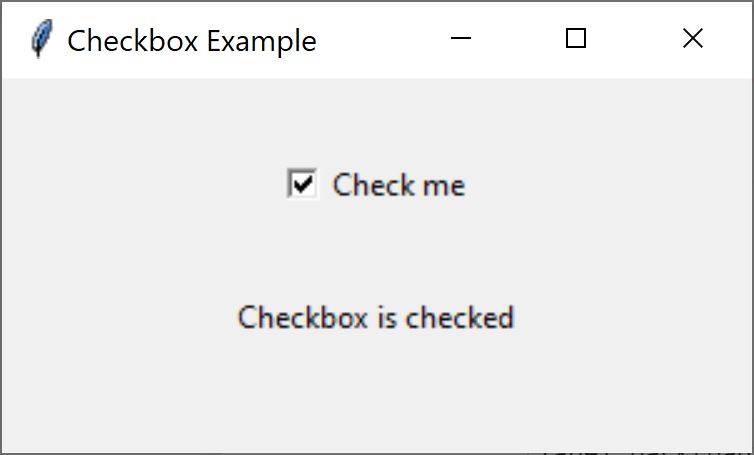
\includegraphics[width=0.6\textwidth]{images/checkbox.JPG}
    \caption{Tkinter}
    \label{fig:checkbox}
\end{figure}


